\chapter{Herramientas}
\label{chap:herramientas}
En este capítulo se van a detallar las herramientas y tecnologías utilizadas en el desarrollo de este proyecto principalmente en el ámbito web. Algunas se han elegido por facilidad de uso y otras por necesidad del entorno desarrollado.

\section{Robot Lego Ev3}
\label{sec:caracteristicas} 
Dentro de los robots de \textit{LEGO} el que más versatilidad, además de más potencia de procesamiento y posibilidades en las opciones de creatividad a la hora de crear robots es \textit{LEGO MINDSTORMS Education}\cite{bib:mindstorm} (Pack en el que viene integrado el \textit{LEGO Ev3}) también trae una mayor gama de sensores, por no decir que es uno de los líderes en la educación STEM (siglas en inglés de Ciencias, Tecnología,Ingeniería y Matemática). En el centro de \textit{LEGO MINDSTORMS Education} se encuentra el Bloque EV3, el bloque inteligente programable que controla motores y sensores y además proporciona comunicación inalámbrica.
 \begin{figure}[H]
    \centering
    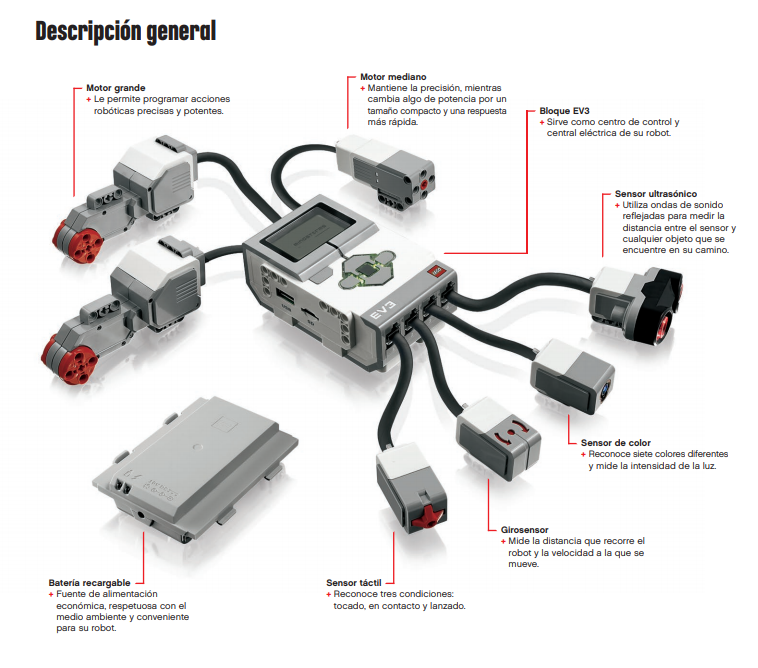
\includegraphics[scale=0.7]{img/partes.png}
    \caption{Conjunto Ev3} \label{fig:partes}
\end{figure}
 Esto quiere decir que las posibilidades a la hora de crear diferentes robots, con diferentes configuraciones de sensores, son prácticamente infinitas. Pero vamos a centrarnos en los casos que más funcionalidad tienen. El robot que más versatilidad presenta a la hora de superar ejercicios, es un robot triciclo, con dos ruedas delanteras y una pivotante trasera. Así que este será nuestro modelo para el robot. Y además, como el \textit{kit de LEGO MINDSTORMS} viene con tres sensores diferentes, crearé tres modelos para integrarlos por separado en la plataforma.

\section{Lenguaje Python}

Python es un lenguaje de programación administrado por la Python Software Foundation.Posee una licencia de código abierto, denominada Python Software Foundation License.Es un lenguaje interpretado, por lo que no se necesita compilar el código fuente para poder ejecutarlo. Esto ofrece ventajas como la rapidez de desarrollo e inconvenientes como una menor velocidad. En ciertos casos, cuando se ejecuta por primera vez un código, se producen unos bytecodes que se guardan en el sistema y que sirven para acelerar la compilación implícita que realiza el intérprete cada vez que se ejecuta el mismo código. 
Este lenguaje nos es muy importante en este proyecto ya que es el lenguaje nativo del robot y en el que van a ir programados los \textit{drivers} para el robot real. 

\section{Lenguaje HTML}

HTML (HyperText Markup Languaje) fue desarrollado en 1991 por Tim Berners-Lee mientras trabajaba en la Organización Europea para la Investigación Nuclear (CERN), y popularizado por el navegador Mosaic desarrollado en NCSA (Raggett, Le Hors y Jacobs, 1999).

Es un lenguaje de marcado que sirve para estructurar una página web. Permite poner etiquetas a diferentes partes de la página para darles la misma apariencia. También tiene tipos de funciones para personalizar el tipo de letra y la forma que tienen en pantalla

Un documento HTML tiene una estructura de árbol  donde la etiqueta html es el elemento raíz y cada nuevo elemento es una rama del anterior. Estas ramas se pueden ir extendiendo sea necesidad del proyecto web.

\begin{lstlisting}[frame=single,breaklines=true, label=Ejemplo de funcionamiento HTTP, caption=Ejemplo de funcionamiento HTTP, captionpos=b]

<!DOCTYPE html>
<html>
  <head>
    <meta charset="utf-8">
    <title>Mi pagina de prueba</title>
  </head>
  <body>
    <img src="images/firefox-icon.png" alt="Mi imagen de prueba">
  </body>
</html>
\end{lstlisting}

HTML5 es la mejora de HTML, establece una serie de nuevos elementos y atributos que reflejan el uso actual de los sitios web modernos, incluye nuevas etiquetas como \texttt{<nav>} que es el bloque de navegación del sitio web. Tiene soporte para \textit{Canvas} y visores para MathML y SVG.\newline

Usare HTML para crear el editor web que se encargará de enviar el código al robot.

\section{Lenguaje JavaScript}
\label{sec:js}
\textit{JavaScript} es un lenguaje de programación interpretado de alto nivel que se encuentra bajo el estándar ECMA Script. Este lenguaje es comúnmente conocido por su uso en los scripts de las páginas web. Es un lenguaje tipado débil y dinámico. Esta diseñado para ser utilizado en páginas Web, actualmente existen otras posibilidades de ejecutar \textit{JavaScript} en todo tipo de aplicaciones haciendo uso de \textit{Nodejs}.\newline
La sintaxis es similar a la utilizada en Java y C++. De esta manera, se facilita el aprendizaje del lenguaje ya que está basado en conceptos ya conocidos por el programador.\newline
Este es el lenguaje en el que estan programados los \textit{drivers} de los robots simulados en la plataforma \textit{Kibotics}. 
% A-FRAME %
\section{Entorno A-Frame}
\label{sec:aframe}
\textit{A-Frame}: \footnote{\url{https://aframe.io/}}  es un entorno de código abierto destinado a crear experiencias de realidad virtual, siendo una de las comunidades creadoras de contenido para realidad virtual más grandes del mundo. Esto se debe a que es un entorno soportado por la mayoria de gafas de VR(\textit{Virtual Reality}) como \textit{OculusRift, HTC Vive o GearsVR}.\newline
\begin{figure}[ht]
    \centering
    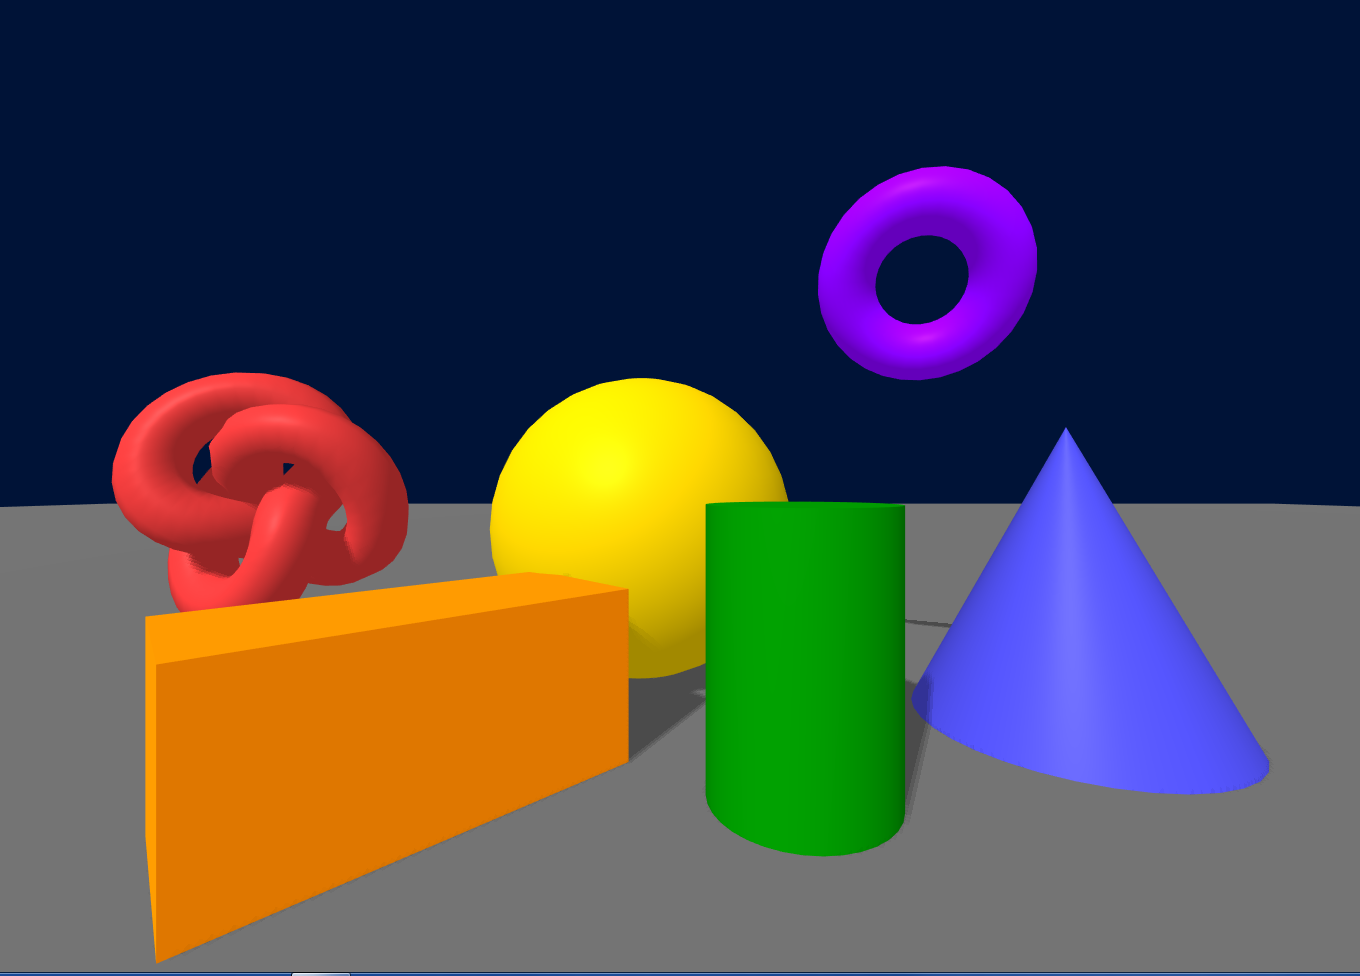
\includegraphics[width=1\textwidth]{img/Aframe.png}
    \caption{Algunos ejemplos de \textit{A-Frame}} 
    \label{fig:A-Frame}
\end{figure}

Esta creado a partir de \textit{HTML} de forma que sea sencillo de leer y comprender. De esta manera es accesible para crear una gran comunidad. \textit{A-Frame} sigue el patrón ECS(entidad-componente-sistema). Se trata de un patrón de desarrollo de juegos basado en el principio de composición sobre herencia. De esta manera, se otorga una mayor flexibilidad en la definición de entidades ya que cada objeto de la escena se corresponde con una entidad y cada entidad,a su vez, está compuesta por uno o más componentes que contienen datos y estado de la entidad. Por tanto, una entidad puede verse modificada en tiempo de ejecución si alguno de los componentes que agrega modifica sus datos.
\\
A-Frame es la base sobre la que esta programado el simulador de la plataforma de \textit{Kibotics}.


% BLENDER %
\section{Editor 3D Blender}
\label{sec:blender}
\textit{Blender} \footnote{\url{https://www.blender.org/}} es un programa libre dedicado al diseño y animación 3D. Mediante una interfaz gráfica permite diseñar objetos, personajes y escenas en tres dimensiones con muy diversas técnicas. Cada uno de los elementos creados pueden ser animados mediante \textit{keyframing} o animación por fotogramas clave. En su origen \textit{Blender} fue distribuido como una herramienta privada explotada por un estudio de animación, pero actualmente se encuentra bajo licencia \textit{GPL} 

    
\begin{figure}[ht]
    \centering
    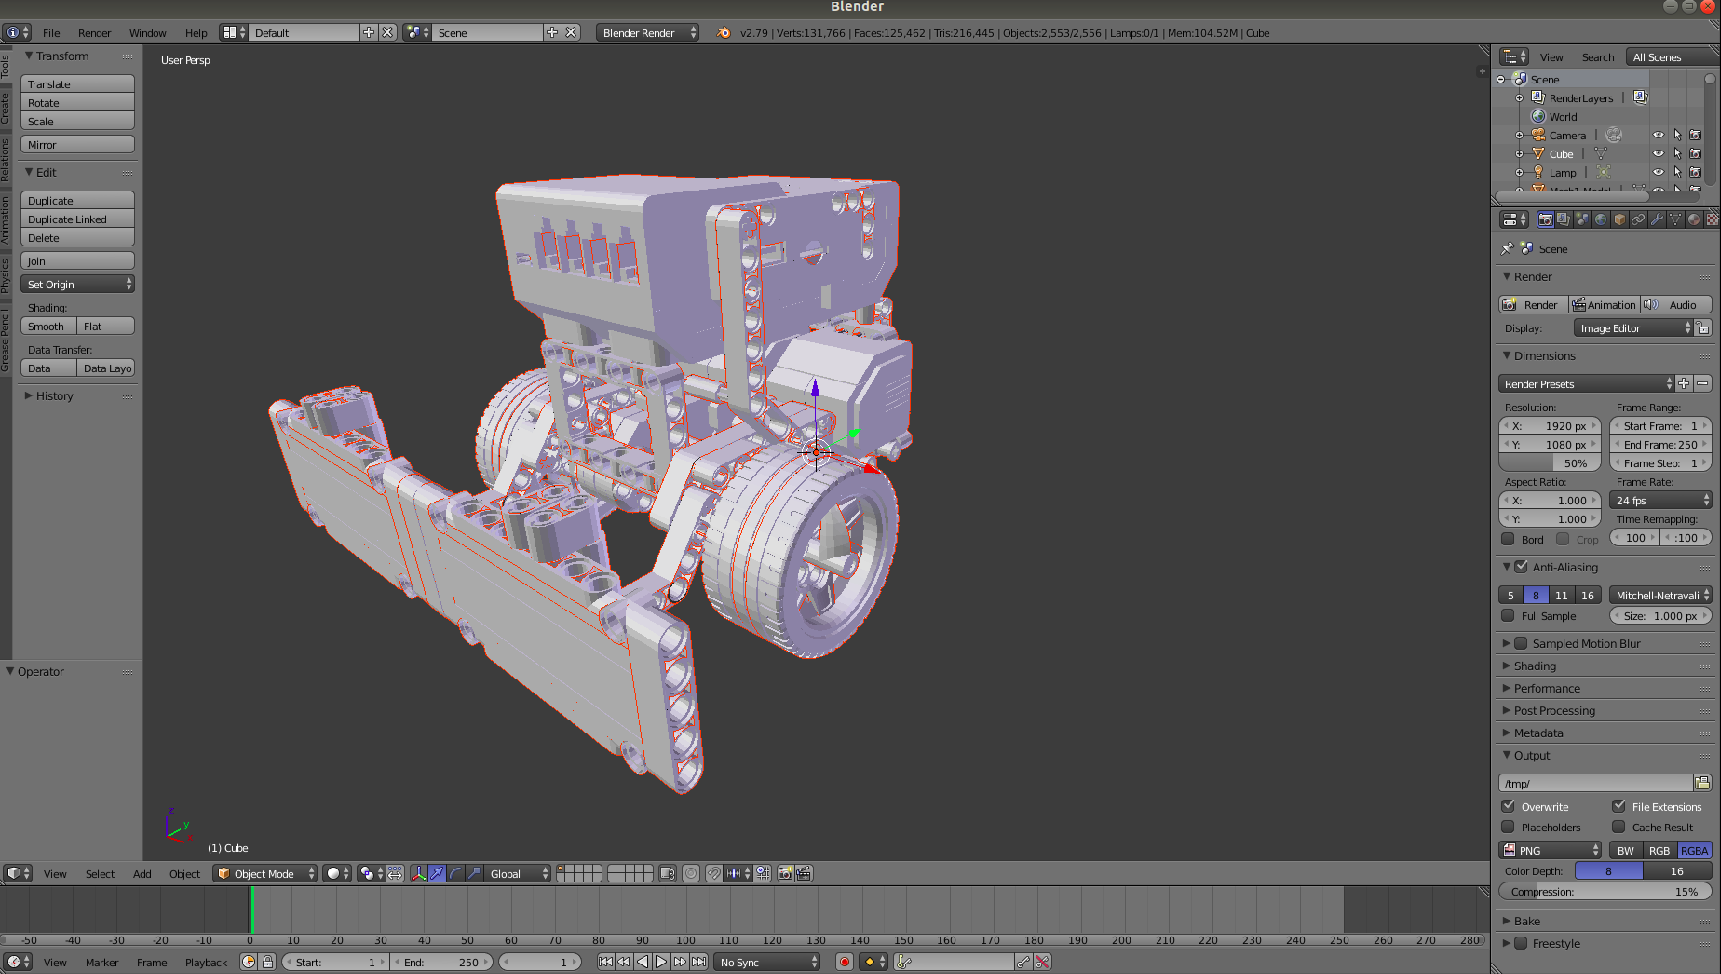
\includegraphics[width=1\textwidth]{img/primermodelo.png}
    \caption{Interfaz gráfica de \textit{Blender}} 
    \label{fig:blender}
\end{figure}

Existe un almacén web desde donde es posible descargarse una gran variedad de modelos y escenarios, además de desarrollar los propios. Una vez desarrollado el modelo o escenario, estos editores exportan el modelo o escenario en formato "gltf", que es un formato soportado por \textit{A-Frame} y estaría listo para insertarlo en el entorno simulado.\newline
Los escenarios y modelos generados por este editor son creados mediante la intersección de líneas, generando los distintos tipos de objetos. Es posible adjuntar una textura o color a cada cara que forma el objeto. Esto lo utilizaré a la hora de crear mis modelos tridimensionales y poder integrarlos en la plataforma \textit{Kibotics}.


% WEBSIM %
\section{Simulador WebSim}

\textit{Websim} es un simulador diseñado para enseñar conceptos básicos de tecnología e iniciar a niños en robótica y programación. 
El simulador hace uso del entorno \textit{A-Frame} y su diseño permite conectar un editor de texto o un editor de bloques para  programar en \textit{JavaScript}, \textit{Blockly} o \textit{Python} y conectar este código con el robot simulado.  En la figura \ref{fig:websim} se puede ver el diseño de \textit{WebSim}.
    

\begin{figure}[H]
    \centering
    \includegraphics[width=1\textwidth]{img/websim.png}
    \caption{Interfaz gráfica de \textit{WebSim}} \label{fig:websim}
\end{figure}

Las características del simulador hacen que los usuarios puedan programar el robot simulado de manera sencilla, ya que solo tengan que acceder a la información que ofrecen los sensores del robot y mandar ordenes a los actuadores. Es decir, que solo tengan que programar la lógica del robot para resolver los ejercicios propuestos. 

El robot consta de sensores simulados con \textit{A-Frame}. Los drivers permiten que el usuario, vía \textit{JavaScript}, pueda acceder a estos y obtener su información. En este entorno disponemos de los siguientes sensores: 

\begin{table}[H]
\caption{Métodos (HAL API) de los sensores del robot.}
\vspace{0.5cm}
\label{tab:tablaSensores}
\resizebox{\textwidth}{!}{%
\begin{tabular}{|c|c|c|ll}
\cline{1-3}
\textbf{Método} & \textbf{Descripción} & \textbf{Salida} &  &  \\ \cline{1-3}
.getDistance() & \begin{tabular}[c]{@{}c@{}}Devuelve la distancia entre el robot\\  y la intersección del raycaster en el centro\end{tabular} & number(metros) &  &  \\ \cline{1-3}
.getDistances() & \begin{tabular}[c]{@{}c@{}}Devuelve la distancia entre el robot y\\ la intersección con cada una de los raycaster\end{tabular} & list number(metros) &  &   \\ \cline{1-3}
.readIR(color) & \begin{tabular}[c]{@{}c@{}}Recorta la imagen, filtra y calcula el centro\\ del objeto con el color pasado como argumento\end{tabular} & number &  &  \\ \cline{1-3}
.getRotation() & \begin{tabular}[c]{@{}c@{}}Retorna un objeto con la orientación \\ del robot en los 3 ejes\end{tabular} & \begin{tabular}[c]{@{}c@{}}\{x:number,\\ y:number,\\ z:number\}\end{tabular} &  &  \\ \cline{1-3}
.getPosition() & Obtiene la posición del robot en la escena & \begin{tabular}[c]{@{}c@{}}\{x:number,\\ y:number,\\ z:number\}\end{tabular} &  &  \\ \cline{1-3}
.getImage() & Devuelve la imagen de la cámara del robot & cv.Mat() &  &  \\ \cline{1-3}
.getObjectColor(color) & \begin{tabular}[c]{@{}c@{}}Devuelve un objeto con la posición del elemento\\ detectado por la cámara del color pasado por parámetro\end{tabular} & \begin{tabular}[c]{@{}c@{}}\{center:{[}x.y{]},\\ area: int\}\end{tabular} &  &  \\ \cline{1-3}
.getObjectColorRGB(valorBajo,valorAlto) & \begin{tabular}[c]{@{}c@{}}Devuelve un objeto con la posición del elemento\\ detectado por la cámara con los valores pasados por parámetro\end{tabular} & \begin{tabular}[c]{@{}c@{}}\{center:{[}x.y{]},\\ area: int\}\end{tabular} &  &  \\ \cline{1-3}
\end{tabular}%
}
\end{table}

Además de sensores, el robot tiene actuadores. Los actuadores se encargan de dar movimiento al robot simulado en \textit{A-Frame}.

En la tabla \ref{tab:tablaMotores} se explican todas las funciones del \textit{HAL API} que hacen referencia a los actuadores.

\begin{table}[H]
  \begin{center}
    \caption{Métodos (HAL API) de los actuadores del robot en \textit{JavaScript}.}
    \vspace{0.5cm}
    \label{tab:tablaMotores}
    \begin{tabular}{|c|c|} 
    \hline
      \textbf{Método} & \textbf{Descripción}\\
      \hline
.setV(integer) & \begin{tabular}[c]{@{}c@{}}Mueve hacia delante o atrás el robot.\\\end{tabular} \\ \hline
.setW(integer) & \begin{tabular}[c]{@{}c@{}}Hace girar al robot.\\\end{tabular} \\ \hline
.move(integer, integer) & \begin{tabular}[c]{@{}c@{}}Mueve el robot hacia delante/atrás y gira al mismo tiempo.\\ \end{tabular} \\ \hline
.getV() & \begin{tabular}[c]{@{}c@{}}Obtener la velocidad lineal configurada en el robot.\\ \end{tabular} \\ \hline
.getW() & \begin{tabular}[c]{@{}c@{}}Obtener la velocidad angular configurada en el robot.\\ \end{tabular} \\ \hline
    \end{tabular}
  \end{center}
\end{table}

Además del \textit{Driver} en \textit{Javascript} para los robots simulados, la plataforma de \textit{Kibotics} ofrece recubrimientos de este HAL API en \textit{Python} y en \textit{Scratch}. Los usuarios programan sus aplicaciones robóticas usando esos interfaces de alto nivel.

\section{Servidor Django}

Django \footnote{\url{https://www.djangoproject.com/es}} un entorno de código abierto escrito en Python, creado en 2005, el cual permite desarrollar un entorno web complejo de una forma rápida y estructurada. Actualmente es mantenido por Django Software Foundation y se encuentra en la versión 3.0, aunque para este proyecto vamos a usar la versión 2.2, que es la que utiliza \textit{Kibotics} actualmente.

Sigue una arquitectura MVC (Modelo – Vista - Controlador), como se observa en la figura.
\begin{itemize}
	\item \textit{Modelo}. Es la representación de la información con la cual el sistema opera, por lo tanto gestiona todos los accesos a dicha información, tanto consultas como actualizaciones, implementando también los privilegios de acceso que se hayan descrito en las especificaciones de la aplicación

	\item \textit{Vista}. Presenta el 'modelo' en un formato adecuado para interactuar (usualmente la interfaz de usuario), por tanto requiere de dicho 'modelo' la información que debe representar como salida.
	
	\item \textit{Controlador}. Responde a eventos e invoca peticiones al 'modelo' cuando se hace alguna solicitud sobre la información.por tanto se podría decir que el 'controlador' hace de intermediario entre la 'vista' y el 'modelo' (.
\end{itemize}
\begin{figure}[h!]
  \centering
    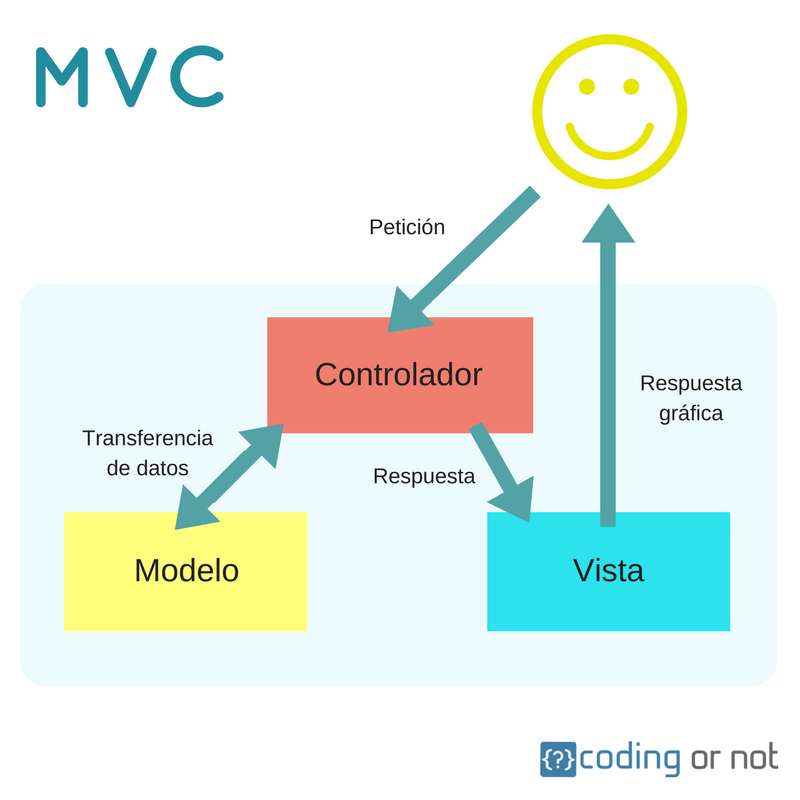
\includegraphics[width=0.6\textwidth]{img/mvc.png}
  \caption{Arquitectura Django}
  \label{Arquitectura Django}
\end{figure}
La meta fundamental de Django es facilitar la creación de sitios web complejos. Django pone énfasis en el re-uso, la conectividad y extensibilidad de componentes, el desarrollo rápido y el principio No te repitas (DRY, del inglés Don't Repeat Yourself). Python es usado en todas las partes del entorno, incluso en configuraciones, archivos, y en los modelos de datos. 


\section{Servidor Flask}

\textit{Flask} \footnote{\url{https://flask.palletsprojects.com/en/1.1.x/}} es un entorno escrito en \textit{Python} y concebido para facilitar el desarrollo de Aplicaciones Web bajo el patrón MVC(Modelo - Vista - Controlador). Se le considera un entrono minimalista porque tiene las herramientas  mínimas necesarias para crear una aplicación web funcional pero si se necesita en algún momento una nueva funcionalidad hay un conjunto muy grande extensiones  que se pueden instalar con \textit{Flask} que le van dotando de funcionalidad.
\begin{figure}[h!]
  \centering
    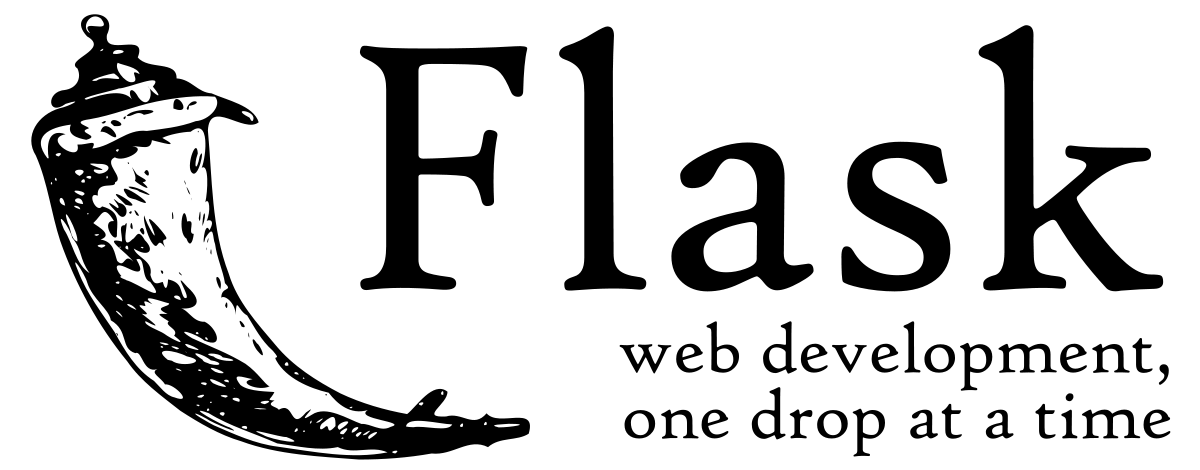
\includegraphics[width=0.4\textwidth]{img/flask.png}
  \caption{Logo Flask}
  \label{Flask}
\end{figure}

Usaré \textit{Flask} para instalar un servidor en el robot \textit{LEGO Ev3} que reciba peticiones.